\section{Revised Block Diagram}

Figure~\ref{fig:blockDiagram} shows a revised system block diagram.  It contains the model numbers of the known components, the types of connection required to the microcontroller unit (MCU) and the amount of lines needed for each connection.  A description of the components not described in the project's proposal follows.

%TODO Fix amount of lines in block diagram
\begin{figure}[H]
	\centering
	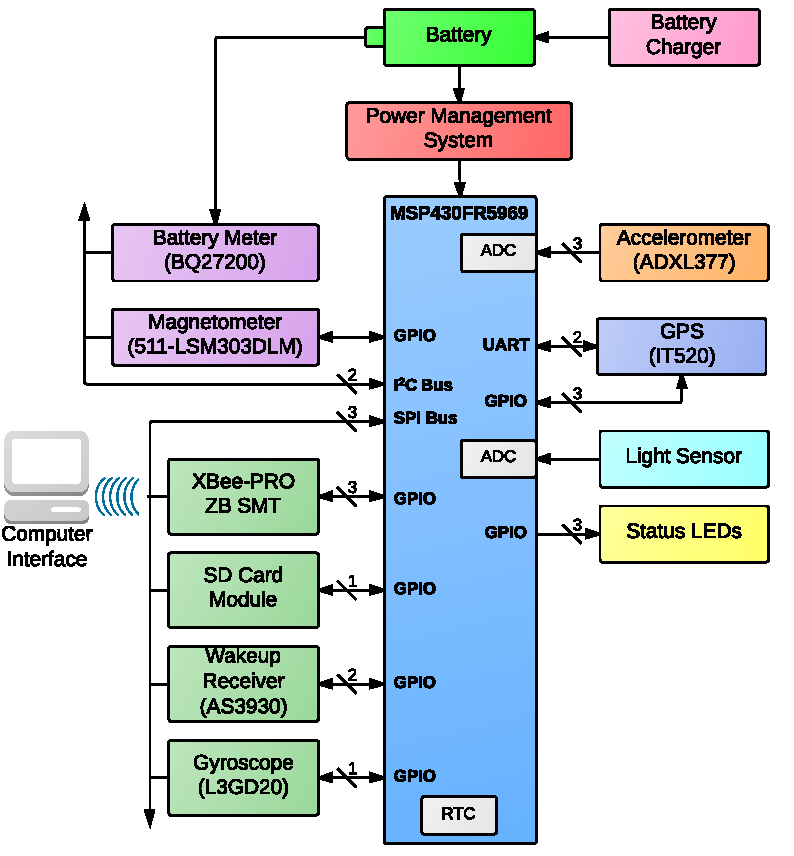
\includegraphics[width=\textwidth]{img/blockDiagramV2_2}
	\caption{Revised Block Diagram \label{fig:blockDiagram}}
\end{figure}

\subsection{RF Wake-Up Receiver}
The RF Wake-Up receiver is a dedicated component that is utilized to wake the MCU from low power mode by issuing an interrupt. The amplitude shifted key (ASK) receiver consumes a very small amount of power while listening for a wake-up signal. This enables the device to be powered on without the need of an external physical button. It also enables the device to operate in Shutdown Mode, where nearly no power is consumed while waiting for user interaction. The idea is to never completely power down the device, but instead leave it in Shutdown Mode which can then be waked up using a low frequency radio identification tag (RFID).

\subsection{Battery Charging and Power Management}
\label{sec:chargingMethods}
Currently, two different methods for charging the sphere's battery are being researched and considered: Wireless Charging and USB Charging.  These methods are described in the following sections.  The descriptions presented are based on the previous decision of using Lithium-Ion or Lithium-Polymer batteries.

Since more research must be done on the wireless charging alternative, it has not yet been chosen definitively.  Because of this, it is difficult to select battery charging and power management circuits since a different charging alternative will change the power management solution that is best suited to the system.  It is important to mention that all the components selected can operate with a supply voltage of 3.3V.

A battery meter has been selected, the BQ27200 from Texas Instruments.  However, if the power management or battery charging solutions contain a component similar to this one, the BQ27200 will not be used in favor of minimizing the space consumed by the integrated circuits.

\subsubsection{Wireless Charger}
Wireless charging involves charging the sphere's battery without being physically connected to an outlet or to another device. The reason this method is being considered is because of convenience. If the device is wirelessly charged, then the device wouldn't need an external port that would be used to charge the battery. Having an external port could be dangerous, since extreme caution must be taken to make sure that the port is waterproof. Another option to charge the battery would require the user to physically open the sphere and charge it with an external charger, which is also inconvenient because the constant opening and closing of the sphere might cause mechanical wear which could lead to water leaks when the sphere is being used. Thus, lack of wireless charging would impose restrictions that would make the sphere less convenient.

The exploration of the idea lead to the discovery of the Qi (pronounced `chee') standard which dictates a wireless charging and communication interface. Qi standards mention that the energy transfer must occur at a distance of up to 40 millimeters and that the primary inductive coil must be flat in a spiral formation \cite{QiStandard}. Because of these constrains the Qi standard was discarded, since it is almost impossible to have a flat coil in the spherical device, while maintaining an axisymmetric design. Furthermore, the standard is intended to be used for multiple devices with different power requirements, thus Qi has a communication protocol that complicates the device and obligates developers to integrate further IC technology that could potentially use more physical board space. 

Discarding Qi lead to the consideration of implementing a custom wireless charger. The basic idea is to transfer energy from a 120V AC outlet trough a transformer into the spheres. The transformer would be two separated coils that can transfer energy at a long distance through electromagnetic induction. An AC current will be created inside the sphere's coil which will then have to be rectified into a DC current that can charge the device's battery. Various factors are to be considered when implementing such charger: energy transfer by inductance is not as efficient as traditional charging methods, the coils require specific geometry and number of turns, and the frequency in which the current changes in the primary coil must be specific, since there is an ideal resonance frequency needed to achieve maximum energy transfer. 

Research, design work and experiments are being performed to converge into an implementation, knowing that it is possible to supply the primary coil with a controlled oscillating DC current that would cause the necessary change in flux to create an inductive charge. Ideally the user will have a charging station that will be connected to a 120V power outlet and can hold a few spheres. Each sphere would then be charged wirelessly without the need of connecting it or opening it.

\subsubsection{USB Charger}
Big effort has been made in recent years to standardize chargers and connectors for music players, cellphones, tablets, and many other consumer electronic products. Micro USB has taken the lead as the standard port for charging the batteries of consumer electronics and manufacturers have dropped their own proprietary connectors to favor the USB standard.

The USB 2.0 standard included the Battery Charging Specification 1.2, which increased the limits of supply current to 1.5A, up from the 500mA the USB 1.0 standard allowed. The USB 3.0 specification allows 900mA of current drawn while concurrently transmitting data. For battery charging, the limit is still 1.5A, even though the Battery Charging specification requires the physical ports themselves to be able to handle 5A.

There are many variables in question when it comes to choosing a battery charger. Different battery technologies need to be charged distinctively. For this application, a technology such as Lithium-Ion or Lithium-Polymer must be used, because Lead-Acid, Nickel-Cadmium, and Nickel-Metal-Hydride batteries are too big, heavy, and do not provide the necessary voltage for this application. It is for this reason also that Li-Ion and Li-Polymer batteries are chosen as the power source for most consumer electronics. Other variables include the number of battery cells that need to be charged and the kind of topology needed to charge the battery. For Lithium-Ion and Lithium-Polymer, two topologies exist: Linear and Switch-mode.

Most handheld devices use a linear charging topology, because it offers many advantages like low implementation cost, design simplicity, and a lower noise operation, when compared to switch-mode, because it has no high frequency switching components. One of the drawbacks of this topology is that it introduces power dissipation in the system. Switch-mode topology offers higher efficiency, but the implementation is more complicated, bulkier, and noisy, which may cause interference. For this application, a linear charging topology is preferred.

After having decided the implementation variables, a charge management controller should be chosen. There are many controllers available commercially. A good example is Microchip's MCP73831/2. This is a single cell, fully integrated Li-Ion and Li-Polymer charge management controller. It uses a linear topology and it is compatible with the standard Micro USB port. Another good example is Texas Instrument's BQ24080. It also uses a linear charge topology, and contains a status indicator pin.

The USB Battery Charging standard is the preferred charging method if the wireless charging option can not be made viable.
